\documentclass{jsarticle}
\title{講義ノート第5回}
\author{}
\date{}


\usepackage[top=30truemm,bottom=30truemm,left=25truemm,right=25truemm]{geometry}

\usepackage{ascmac}

\usepackage{amsmath}

\usepackage[dvips]{graphicx}

\usepackage{ulem}

\parindent = 0pt

\begin{document}
\maketitle

\section{静電場}

\setcounter{subsection}{10}

\subsection{静電ポテンシャル}
\subsubsection{静電場は渦を持つか?}
空間の任意の位置に電荷$q_i(i=1,2,3...)$が固定された静電場の式は,
\begin{eqnarray}
{\bf E}({\bf r})=\sum_i \frac{q_i}{4 \pi \varepsilon_0} \frac{{\bf r}-{\bf r}_i}{|{\bf r}-{\bf r}_i|^3}
\end{eqnarray}
この静電場の回転は,回転の線形性から,各電荷による電場の回転の重ね合わせとなる.
\begin{eqnarray}
{\rm rot}{\bf E} = \sum_i  {\rm rot} \left( \frac{q_i}{4 \pi \varepsilon_0} \frac{{\bf r}-{\bf r}_i}{|{\bf r}-{\bf r}_i|^3} \right) 
= \sum_i \frac{q_i}{4 \pi \varepsilon_0} {\rm rot} \left( \frac{{\bf r}-{\bf r}_i}{|{\bf r}-{\bf r}_i|^3} \right)
\end{eqnarray}
${\bf r}=(x,y,z), {\bf r}_i = (x_i,y_i,z_i)$ \\
$|{\bf r}-{\bf r}_i|=\sqrt[]{\mathstrut (x-x_i)^2+(y-y_i)^2+(z-z_i)^2}=R$とすると,
\begin{eqnarray}
{\rm rot}\left( \frac{{\bf r}-{\bf r}_i}{|{\bf r}-{\bf r}_i|^3} \right) =
{\rm rot}
\left( 
\begin{array}{cc}
\frac{x-x_i}{R^3} \\
\\
\frac{y-y_i}{R^3} \\
\\
\frac{z-z_i}{R^3} \\
\end{array}
\right)
=
\left( 
\begin{array}{cc}
\frac{\partial}{\partial y} \left( \frac{z-z_i}{R^3} \right) -\frac{\partial}{\partial z} \left( \frac{y-y_i}{R^3} \right) \\
\\
\frac{\partial}{\partial z} \left( \frac{x-x_i}{R^3} \right) -\frac{\partial}{\partial x} \left( \frac{z-z_i}{R^3} \right) \\
\\
\frac{\partial}{\partial x} \left( \frac{y-y_i}{R^3} \right) -\frac{\partial}{\partial y} \left( \frac{x-x_i}{R^3} \right) \\
\end{array}
\right)
\end{eqnarray}
z成分だけ計算する.
\begin{eqnarray}
\mbox{z成分} &=&(y-y_i) \frac{\partial}{\partial x} \left( \frac{1}{R^3} \right) - (x-x_i) \frac{\partial}{\partial y} \left( \frac{1}{R^3} \right) \\
&=& -3(y-y_i) \frac{1}{R^4}\frac{\partial R}{\partial x} + 3(x-x_i) \frac{1}{R^4}\frac{\partial R}{\partial y}
\end{eqnarray}
$\frac{\partial R}{\partial x}=\frac{x-x_i}{R}$,$\frac{\partial R}{\partial y}=\frac{y-y_i}{R}$より,
\begin{eqnarray}
\mbox{z成分}= -3(y-y_i) \frac{x-x_i}{R^5} + 3(x-x_i) \frac{y-y_i}{R^5} = 0
\end{eqnarray}
他の成分も同様に0となる.したがって
\begin{itembox}[c]{静電場の回転}
\begin{eqnarray}
{\rm rot}{\bf E} = {\bf 0} \mbox{(静電場は渦なし)}
\end{eqnarray}
\end{itembox}
静電場に渦がないことを直観的に理解するには,1つの点電荷に注目すればよいが,これは明らかに渦なしと分かる.(図1)すると静電場には重ね合わせの原理が成り立つから,任意の静電場に対して回転が0となり,渦なしであることが分かる.\\
\begin{figure}[htbp]
 \begin{center}
  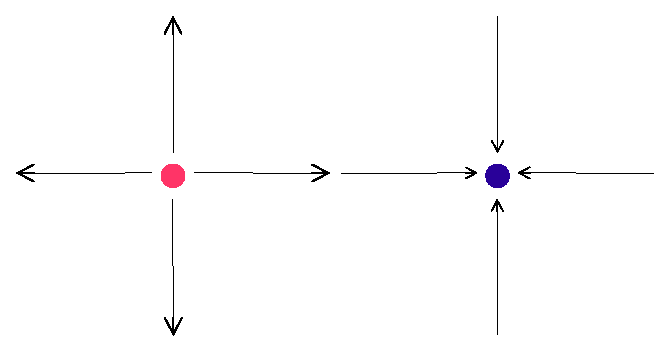
\includegraphics[width=80mm]{5.1.eps}
 \end{center}
 \caption{}
 \label{fig:one}
\end{figure}
式(7)はMaxwell方程式のひとつを静電場の場合に適応したものとなっている.ただし,電場が時間に依存する場合にはその式に補正が入る.(後述)

\subsubsection{線積分は経路に依存するか?}
\begin{figure}[htbp]
 \begin{center}
  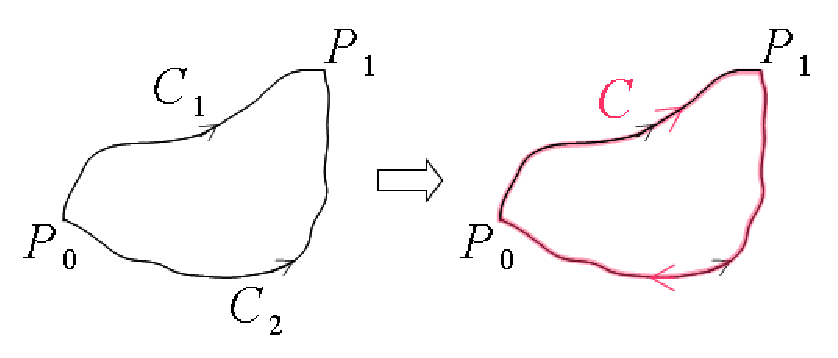
\includegraphics[width=150mm]{5.2.eps}
 \end{center}
 \caption{}
 \label{fig:two}
\end{figure}
\begin{figure}[htbp]
 \begin{center}
  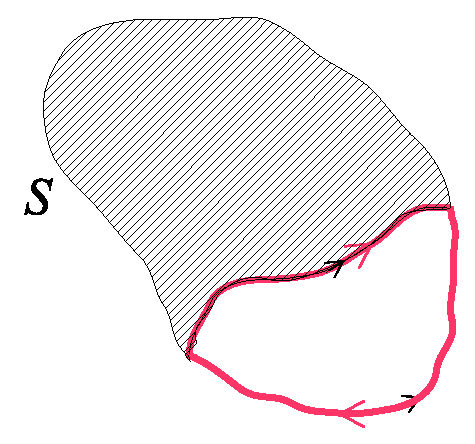
\includegraphics[width=50mm]{5.3.eps}
 \end{center}
 \caption{}
 \label{fig:three}
\end{figure}
$P_0$から$P_1$に向かう異なる経路$C_1$,$C_2$について,電場{\bf E}の線積分の差をとる.
\begin{eqnarray}
\int_{C_1}^{} {\bf E} \cdot {\bf dl} - \int_{C_2}^{} {\bf E} \cdot {\bf dl}
\end{eqnarray}
ここで$- \int_{C_2}^{} {\bf E} \cdot {\bf dl}=\int_{C_2}^{} {\bf E} \cdot {-\bf dl}$に着目すると,これは$P_1$から$P_0$に向かう経路$C_2$に沿った電場の線積分となっている.したがって$\int_{C_1}^{} {\bf E} \cdot {\bf dl}$と方向に注意して経路をつなげると,図2のような有向ループ$C$に沿った線積分となる.よって
\begin{eqnarray}
\int_{C_1}^{} {\bf E} \cdot {\bf dl} - \int_{C_2}^{} {\bf E} \cdot {\bf dl} = \int_{C}^{} {\bf E} \cdot {\bf dl}
\end{eqnarray}
ここで,有向ループCをふちにもつ任意の曲面Sをとると,Stokesの定理より,
\begin{eqnarray}
\int_{C}^{} {\bf E} \cdot {\bf dl} = \int_{S}^{} {\rm rot}{\bf E} \cdot {\bf dS} \mbox{(面積分)}
\end{eqnarray}
もう一度繰り返すが,静電場は渦なしだから,
\begin{eqnarray}
\int_{S}^{} {\rm rot}{\bf E} \cdot {\bf dS} = \int_{S}^{}  {\bf 0} \cdot {\bf dS} = 0
\end{eqnarray}
よって
\begin{eqnarray}
\int_{C_1}^{} {\bf E} \cdot {\bf dl} = \int_{C_2}^{} {\bf E} \cdot {\bf dl}
\end{eqnarray}
となり,静電場の線積分は,端点の位置のみにより,途中の経路によらないことがわかる.\\
特に,ループ(閉路)についての線積分はループの形によらず0となる.\\
\subsubsection{静電ポテンシャル(電位)}
さて,スカラー場$\phi$({\bf 静電ポテンシャル}あるいは{\bf 電位}と)を以下のように定義する.
\begin{itembox}[c]{{\bf 静電ポテンシャル}({\bf 電位})}
\begin{eqnarray}
\phi = - \int_{P_0}^{{\bf r}} {\bf E} \cdot {\bf dl}
\end{eqnarray}
$P_0$は$\phi(P_0)=0$となるように選ぶ.{\bf r}は任意の位置である. \\
線積分は$P_0 \to {\bf r}$の経路によらないので,端点のみで指定する定積分は意味を持つ.
\end{itembox}
ではどのような意味を持つか. \\
次元は,$[\phi] = [{\bf E}] \times [\mbox{長さ}] = \frac{N}{C} \cdot m = \frac{J}{C}$ \\
よって電位はエネルギーと結びついていることが分かる. 
\newpage
\begin{figure}[h]
 \begin{center}
  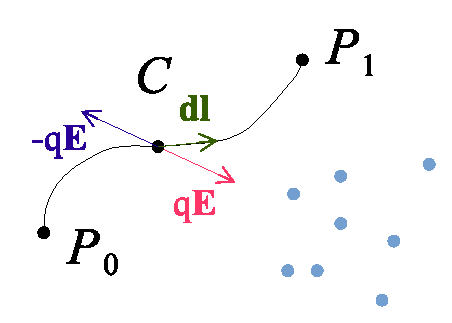
\includegraphics[width=80mm]{5.4.eps}
 \end{center}
 \caption{}
 \label{fig:four}
\end{figure}
電場{\bf E}の中を$P_0$から$P_1$まで,経路Cに沿って電荷$q$を移動するには,経路の各点で電場による力$q{\bf E}$を相殺するように$-q{\bf E}$の力をかけて行う. \\
それに要する仕事は
\begin{eqnarray}
\int_{C}^{} (-q{\bf E}) \cdot {\bf dl} = -q \int_{P_0}^{P_1} {\bf E} \cdot {\bf dl} = q \left( \phi (P_1) - \phi (P_0) \right) = q \phi (P_1)
\end{eqnarray}
{\bf 例}  \\
\begin{figure}[htbp]
 \begin{center}
  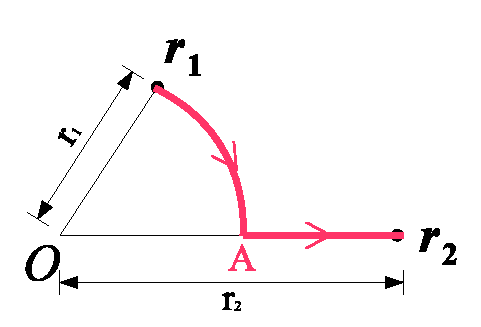
\includegraphics[width=80mm]{5.5.eps}
 \end{center}
 \caption{}
 \label{fig:five}
\end{figure}
原点Oに点電荷$q$を固定する. \\
有向経路に沿った,電場の線積分は,
\begin{eqnarray}
\int_{{\bf r}_1 \to A \to {\bf r}_2}^{} {\bf E} \cdot {\bf dl} = \int_{{\bf r}_1 \to A}^{} {\bf E} \cdot {\bf dl} + \int_{A \to {\bf r}_2}^{} {\bf E} \cdot {\bf dl}
\end{eqnarray}
${\bf r}_1 \to A$ の区間は{\bf E}と{\bf dl} が常に直交するから,$\int_{{\bf r}_1 \to A}^{} {\bf E} \cdot {\bf dl} = 0$ \\
$A \to {\bf r}_2$ の区間は明らかで,
\begin{eqnarray}
\int_{A \to {\bf r}_2}^{} {\bf E} \cdot {\bf dl} = \int_{r_1}^{r_2} \frac{q}{4 \pi \varepsilon_0 l^2} dl = \frac{q}{4 \pi \varepsilon_0} \left( \frac{1}{r_1}-\frac{1}{r_2} \right)
\end{eqnarray}
次に,位置${\bf r_1}$と位置${\bf r_2}$の電位の差を求める.電位が0になる基準の点を$P_0$とすると,
\begin{eqnarray}
 \phi ({\bf r}_1) - \phi ({\bf r}_2) &=& - \int_{P_0}^{{\bf r}_1} {\bf E} \cdot {\bf dl} - \left( -\int_{P_0}^{{\bf r}_2} {\bf E} \cdot {\bf dl} \right) \\
&=& \int_{{\bf r}_1}^{P_0} {\bf E} \cdot {\bf dl} + \int_{P_0}^{{\bf r}_2} {\bf E} \cdot {\bf dl} 
= \int_{{\bf r}_1}^{{\bf r}_2} {\bf E} \cdot {\bf dl} 
\end{eqnarray}
{\bf 原点に1個の点電荷qがある場合} \\
\begin{eqnarray}
\left \{
\begin{array}{l}
{\bf r}_1 = {\bf r} \\
|{\bf r}|=r \\
r_2 \to \infty 
\end{array}
\right.
\end{eqnarray}
とすると,無限遠$\infty$を基準点とする電位は,$\phi(\infty)=0$となるから,
\begin{eqnarray}
\phi ({\bf r}) = \frac{q}{4 \pi \varepsilon_0 r}
\end{eqnarray}
\begin{figure}[htbp]
 \begin{center}
  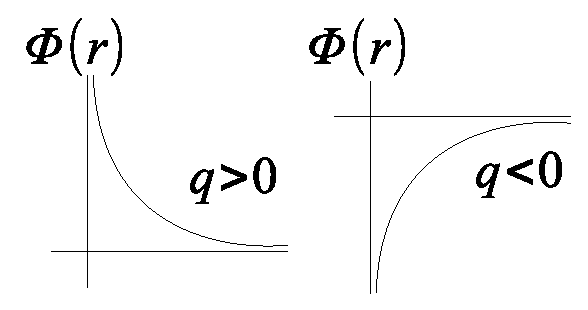
\includegraphics[width=100mm]{5.6.eps}
 \end{center}
 \caption{}
 \label{fig:six}
\end{figure}
\\
{\bf 点電荷集団の場合} \\
(${\bf r}_i$に$q_i$を固定) \\
電場について重ね合わせの原理が成り立つため,電位についても重ね合わせの原理が成り立ち, $\phi(\infty) = 0$とすると,
\begin{eqnarray}
\phi ({\bf r}) = \sum_i \frac{q_i}{4 \pi \varepsilon_0 |{\bf r}-{\bf r}_i|}
\end{eqnarray}
さて,電位と電場はどのような関係によって結ばれているか. \\
そのために位置${\bf r}$と,そこからわずかに移動した位置${\bf r}+{\bf \delta {\bf r}}$ の電位差を考える. \\
まず式(17),(18)から,
\begin{eqnarray}
\phi ({\bf r}+{\bf \delta {\bf r}}) - \phi({\bf r}) = - \int_{{\bf r}}^{{\bf r}+{\bf \delta {\bf r}}} {\bf E} \cdot {\bf dl}
\end{eqnarray}
左辺で,$\delta {\bf r}$は微小変位だから,${\bf \delta {\bf r}}$の2次以上の補正項を無視すると,
\begin{eqnarray}
\phi ({\bf r}+{\bf \delta {\bf r}}) - \phi({\bf r}) = \phi (x+ \delta x, y + \delta y, z + \delta z) - \phi(x,y,z) \simeq \frac{\partial \phi}{\partial x} \delta x + \frac{\partial \phi}{\partial y} \delta y + \frac{\partial \phi}{\partial z} \delta z
\end{eqnarray}
右辺で,$\delta {\bf r}$は微小変位だから,電場を位置${\bf r}$で代表させて線積分すると,
\begin{eqnarray}
- \int_{{\bf r}}^{{\bf r}+{\bf \delta {\bf r}}} {\bf E} \cdot {\bf dl} \simeq - {\bf E} \cdot {\bf \delta r} = - E_x \delta x - E_y \delta y - E_z \delta z
\end{eqnarray}
${\bf \delta r}$が任意の微小変位であるから,両辺の係数を比較して,
\begin{eqnarray}
E_x = - \frac{\partial \phi}{\partial x}, E_y = - \frac{\partial \phi}{\partial y}, E_z = - \frac{\partial \phi}{\partial z}
\end{eqnarray}
さて,任意のスカラー場Vの{\bf 勾配(gradient)}を以下のように定義する. \\
\begin{itembox}[c]{スカラー場Vの{\bf 勾配}}
\begin{eqnarray}
{\rm {\bf grad}}\,V =
\left(
\begin{array}{l}
\frac{\partial V}{\partial x} \\
\\
\frac{\partial V}{\partial y} \\
\\
\frac{\partial V}{\partial z}
\end{array}
\right)
\end{eqnarray}
\end{itembox}
すると電場と電位の関係は以下のように書ける.
\begin{itembox}[c]{電場と電位の関係}
\begin{eqnarray}
{\bf E} = - {\rm{\bf grad}}\, \phi
\end{eqnarray}
\end{itembox}
{\bf 例} \\
原点に1つの点電荷がある場合,$r=\sqrt[]{\mathstrut x^2+y^2+z^2}$とすると,電位は,$\phi=\frac{q}{4 \pi \varepsilon_0 r}$ となる.\\
勾配の$x$成分に-を掛けたものは, \\
\begin{eqnarray}
-({\rm {\bf grad}}\, \phi)_x = - \frac{\partial \phi}{\partial x} &=& -\frac{q}{4 \pi \varepsilon_0} \frac{\partial}{\partial x} \left( \frac{1}{r} \right) \\
&=& \frac{q}{4 \pi \varepsilon_0} \frac{x}{r^3} = \left( \frac{q}{4 \pi \varepsilon_0} \frac{{\bf r}}{r^3} \right)_x \\
&=&E_x
\end{eqnarray}
\subsubsection{等電位面}
電位が$\phi(x,y,z)=\phi_0$,つまり一定値をとる面を,{\bf 等電位面}という. \\
電位$\phi$となる等電位面は,その勾配${\bf grad} \phi$に垂直となる. \\
また,勾配の符号を変えたものが電場であるから,電場も等電位面に垂直になる.
\begin{eqnarray}
{\bf grad}\, \phi \perp \mbox{等電位面} \\
{\bf E} \perp \mbox{等電位面}
\end{eqnarray}
\begin{figure}[htbp]
 \begin{center}
  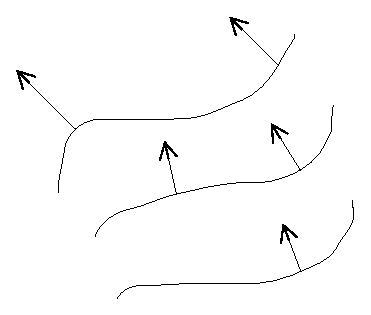
\includegraphics[width=50mm]{5.7.eps}
 \end{center}
 \caption{}
 \label{fig:seven}
\end{figure}
{\bf 例}\footnote{ここからは第6回の内容ですが,切りの都合で続けて書かせて頂きます.} \\
原点に1つの点電荷がある場合,
\begin{figure}[h]
 \begin{center}
  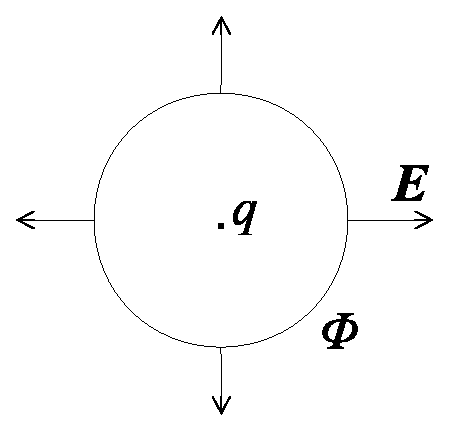
\includegraphics[width=50mm]{5.8.eps}
 \end{center}
 \caption{}
 \label{fig:eight}
\end{figure}
電位は$\phi=\frac{q}{4 \pi \varepsilon_0 r}$であるため,等電位面は,点電荷を中心とする球面となる.したがって電場は等電位面と垂直となる. \\
任意の静電場について,$\mbox{等電位面} \perp {\bf E}$となることを証明する. \\
{\bf 証明} \\
\begin{figure}[htbp]
 \begin{center}
  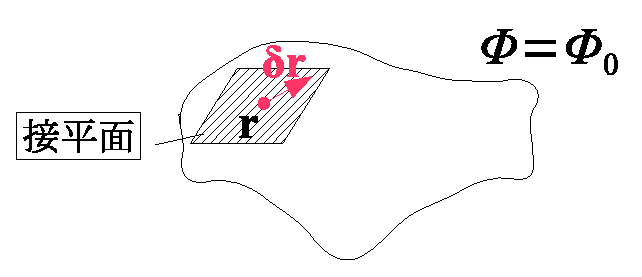
\includegraphics[width=100mm]{5.9.eps}
 \end{center}
 \caption{}
 \label{fig:nine}
\end{figure}
ある等電位面上の位置${\bf r}$と,そこからわずかにずれた位置${\bf r}+{\bf \delta r}$の間の電位差は, \\
\begin{eqnarray}
\phi ({\bf r}+{\bf \delta {\bf r}}) - \phi({\bf r}) &=& \delta x \frac{\partial \phi}{\partial x} + \delta y \frac{\partial \phi}{\partial y} + \delta z \frac{\partial \phi}{\partial z} + \left(
\begin{array}{l}
\mbox{${\bf \delta r}$についての} \\
\mbox{2次以上の補正}
\end{array}
\right) \\
&=&{\bf \delta r} \cdot {\bf grad}\, \phi + \left(
\begin{array}{l}
\mbox{${\bf \delta r}$についての} \\
\mbox{2次以上の補正}
\end{array}
\right)
\end{eqnarray}
変位を表すベクトル${\bf \delta r}$を等電位面に対する接平面内に取ると,${\bf \delta r}$についての1次の項は消え, \\
\begin{eqnarray}
\phi ({\bf r}+{\bf \delta {\bf r}}) - \phi({\bf r}) = 0 + \left(
\begin{array}{l}
\mbox{${\bf \delta r}$についての} \\
\mbox{2次以上の補正}
\end{array}
\right)
\end{eqnarray}
となる.よって${\bf \delta r}$が接平面内(とみなせる)ならば,
\begin{eqnarray}
{\bf \delta r} \cdot {\bf grad}\, \phi = 0 \Leftrightarrow {\bf \delta r} \perp {\bf grad}\, \phi \Leftrightarrow \mbox{接平面} \perp {\bf E}
\end{eqnarray}
\begin{flushright}
(証明終)
\end{flushright}
\end{document}